\documentclass{article}
\usepackage{amsmath}
\usepackage{amssymb}
\usepackage[parfill]{parskip}
\usepackage[utf8]{inputenc}
\usepackage{graphicx}
\usepackage{subfig}
\usepackage{listings}
\graphicspath{{image/}}

%Russian-specific packages
%--------------------------------------
\usepackage[T2A]{fontenc}
\usepackage[utf8]{inputenc}
\usepackage[russian]{babel}
%--------------------------------------

\usepackage[a4paper, total={7in, 10.5in}]{geometry}

\author{Kupriyanov Kirill}
\title{Data Analysis PI\\Theoretical assignment $\#8$}
\date{}

\begin{document}
\maketitle
\thispagestyle{empty}
\newpage

\maketitle

\paragraph{Problem 1}\mbox{}\\

Assume that the AdaBoost classification algorithm is trained on the dataset below. The weak classifiers
set includes decision rules of the form $f(x_1, x_2) = sign(x_i < \theta), i = 1, 2$ (weak classifiers are decision
trees with depth = 1).


(a) Explain, what weak classifier will be obtained after the first iteration.

(b) What object (s) will have the largest weight after the first iteration? What is this weight value?

(c) Explain, what weak classifier will be obtained after the second iteration.

(d) Is it possible to choose the linear coefficients for these two weak classifiers such that their linear
combination would classify the dataset with no errors?

\paragraph{Solution 1}\mbox{}

(a) the first iteration will produce a split as shown in figure 1:
So as precisely it has the greatest criterion Jeannie.



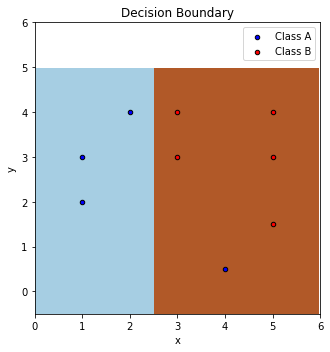
\includegraphics[width=6cm] {1.png}

(b) The highest weight will be given to the element on which the first algorithm is wrong, it is the element (4, 0.5)

(с) the Second algorithm will make the sample as in the picture 2


\includegraphics[width=6cm] {2.png}

(d) Yes, it is possible, if we assign a weight greater than the first to the second classifier, we will achieve an error-free classification, since the 2 algorithm corrects the error of the first one.


\paragraph{Problem 2}\mbox{}\\

Assume that we train the gradient boosting with decision trees as weak classifiers and the loss function $\mathcal{L}(y_i, \hat y_i) = \exp (-y_i\hat y_i)$. What labels should we use for training of a tree on the particular iteration if
the current sum of the trained trees produces a vector of predicted labels $\hat y$?

\paragraph{Solution 2}\mbox{}

In classification problems, we always try to maximize the accuracy of our prediction, but since such loss is not differentiable, we have to use differentiable loss. For example, $\exp (-y_i\hat y_i)$.
The final task is to create a function $a_n (x)$ that minimizes the total error:
$\sum_{i=0}^n\mathcal{L}(y_i, a_N(x_i)) = \sum_{i=0}^n \exp(-y_i a_N(x_i)) \rightarrow \min$. Let $y_i$  - take the values  $\{C_1, C_2\}$,  it is obvious that  $C_1 \neq C_2$,  because it would not distinguish classes at all. Also without prejudice to the generality, we may assume that $C_1 \neq 0$. Then $\mathcal{L}(\{C_1,C_2\},a_N(x_j)) =
\exp(-\{C_1, C_2\}  a_N(x_j)) =
\exp(-\{1, C_2 / C_1\}a_N(x_j))^{C_1}$ the optimum of this error is the same as the error of the form  $\exp(-\{1, C_2 / C_1\}a_N(x_j)), C_1 > 0$.  It turns out that inappropriate generalities can be used to label $\{1, C\}$. Then you can see that when $C > 0$ the algorithm $a_N(x)$ will try to give the most large responses to all classes indiscriminately, as $\underset{a_N(x)}{min} \exp(-{1,C>0}a_N(x)) \rightarrow a_N(x) = +\infty$.
 So it becomes obvious that the use of class labels of the form $\{1, C=0\}$ is incorrect, because the responses of the type $(0, 1)$, $(0, 0)$, $(1, 0)$ - the loss will be the same, which we would not like.
Thus it is possible to come to labels like $\{1, C<0\}$. Such labels will be exponentially much to penalize the algorithm if he is confident in their wrong answer, but not to encourage him in his strong confidence in the correct answer. As the selection of constants C can be used to increase the penalties for error on the highlighted class.


\paragraph{Problem 3}\mbox{}\\

Consider linear regression model with $d$ features $g(x_1, x_2, \dots , x_d)$ and partial dependency plot of feature
$x_i: \phi(x_i)$. Show that partial dependency plot for linear regression provides visualization of weight for feature $x_i$.



\paragraph{Solution 3}\mbox{}

PDP is a graph of the dependence of the algorithm response when some variable $x_i$ is variable, other variables can be taken from the original dataset. But since every linear model is described as follows: $d (X_j) = <w, X_j> + b$, thus the output PDP will get a set of points located on a single line. Since if you pin all variables except $x_i$ - we get some linear function of the form: $\phi(x_i) = a_i * x_i + b$. This function on the chart will carry the iformation of the variable $a_i$ as it will depend on the slope of the line. So PDP is capable of visualizing the weight of a variable on linear models.

\end{document}
